\chapter{Background} \label{ch:background}
\epigraph{From now on you shall be called Brian that is called Brian.}{The Life of Brian}
In this chapter, we introduce commonly used formalisms and definitions.

\section{\acrlong{fol}}
\begin{figure}[t]
  \centering
  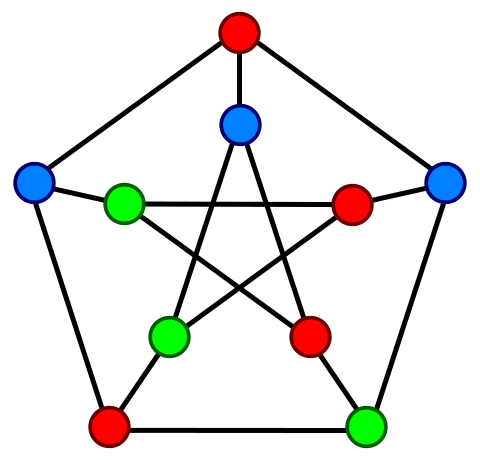
\includegraphics[width=0.4\textwidth]{Petersen_graph_coloring.png}
  \caption{Graph coloring of the Petersen's graph using three colors}
  \label{fig:petersen_coloring}
\end{figure}
In this section, we describe the syntax and semantics of \acrshort{fol},
for an extensive overview of \acrshort{fol}, we refer to \textcite{fo_overview}.

A formal language is a triple: \textit{vocabulary}, \textit{syntax} and \textit{semantics}. Vocabulary is the set of symbols that can be used. Syntax is the set of rules on how these symbols can be combined together. And semantics is the way to interpret the statements.

For each predicate $p$ and each function symbol $f$ in the vocabulary, we assume a natural number $n$ called \textit{arity} to be given, written as $p/n$ and $f/n$. This number indicates the number of parameters it takes, we often omit the arity if it is clear from the context. Propositional symbols are zero-arity predicates and constants are zero-arity functions. 
We assume propositional symbols \textit{true}, $\top$ and \textit{false}, $\bot$ to be always in the vocabulary.

\begin{example}[Predicates and functions]
  Consider the famous problem of coloring a map, as in Figure \ref{fig:petersen_coloring}. The vocabulary would contain a predicate symbol \textit{border/2} and a function \textit{coloring/1}, together with a set of constants representing countries, such as \textit{belgium}, \textit{netherlands}, etc.
\end{example}

\paragraph{Syntax} 


\paragraph{Semantics}


\section{\acrlong{asp}}

\section{FO$(\cdot)$ and the IDP system}

\section{Inductive Logic Programming and Relational Pattern Mining}
